\documentclass[tikz,border=8pt]{standalone}
\usepackage{tikz}
\usepackage{pgfplots}
\usepackage{amsmath,amssymb}
\usepackage[T1]{fontenc}
\usepackage{lmodern}
\usepackage{xcolor}
\usetikzlibrary{arrows.meta,positioning,shapes.geometric,fit,calc,backgrounds,matrix}
\pgfplotsset{compat=1.18}
\definecolor{ink}{HTML}{18202A}
\definecolor{blue}{HTML}{2563EB}
\definecolor{bluefill}{HTML}{EAF1FF}
\definecolor{green}{HTML}{14804A}
\definecolor{greenfill}{HTML}{E8F6EE}
\definecolor{amber}{HTML}{B56A00}
\definecolor{amberfill}{HTML}{FFF3D6}
\definecolor{red}{HTML}{B42318}
\definecolor{redfill}{HTML}{FDECEC}
\definecolor{gray}{HTML}{667085}
\definecolor{light}{HTML}{F4F6F8}
\definecolor{linegray}{HTML}{C7CDD4}
\tikzset{
  box/.style={draw=ink, rounded corners=3pt, very thick, fill=white, align=center, inner sep=7pt, font=\sffamily\small},
  bluebox/.style={box, fill=bluefill, draw=blue},
  greenbox/.style={box, fill=greenfill, draw=green},
  amberbox/.style={box, fill=amberfill, draw=amber},
  redbox/.style={box, fill=redfill, draw=red},
  ghost/.style={draw=linegray, rounded corners=3pt, thick, fill=light, align=center, inner sep=7pt, font=\sffamily\small},
  label/.style={font=\sffamily\footnotesize, text=gray, align=center},
  title/.style={font=\sffamily\bfseries\large, text=ink, align=center},
  arrow/.style={-{Latex[length=3mm,width=2mm]}, very thick, draw=ink},
  bluearrow/.style={-{Latex[length=3mm,width=2mm]}, very thick, draw=blue},
  redarrow/.style={-{Latex[length=3mm,width=2mm]}, very thick, draw=red},
  greenarrow/.style={-{Latex[length=3mm,width=2mm]}, very thick, draw=green}
}

\begin{document}
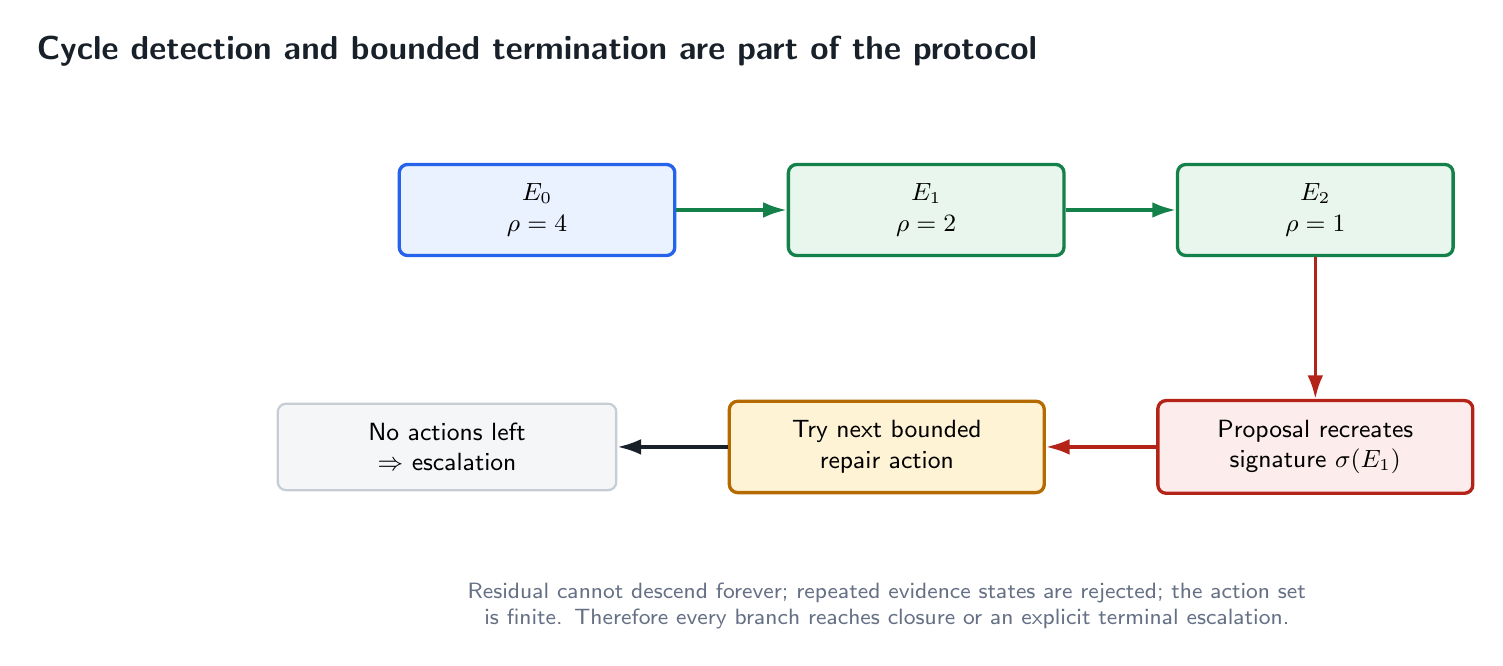
\begin{tikzpicture}[node distance=13mm and 14mm]
\node[title] (ttl) {Cycle detection and bounded termination are part of the protocol};
\node[bluebox, below=11mm of ttl, minimum width=35mm] (s0) {$E_0$\\$\rho=4$};
\node[greenbox, right=of s0, minimum width=35mm] (s1) {$E_1$\\$\rho=2$};
\node[greenbox, right=of s1, minimum width=35mm] (s2) {$E_2$\\$\rho=1$};
\draw[greenarrow] (s0)--(s1); \draw[greenarrow] (s1)--(s2);
\node[redbox, below=18mm of s2, minimum width=40mm] (rep) {Proposal recreates\\signature $\sigma(E_1)$};
\draw[redarrow] (s2)--(rep);
\node[amberbox, left=of rep, minimum width=40mm] (next) {Try next bounded\\repair action};
\draw[redarrow] (rep)--(next);
\node[ghost, left=of next, minimum width=43mm] (term) {No actions left\\$\Rightarrow$ escalation};
\draw[arrow] (next)--(term);
\node[label, below=10mm of next, text width=130mm] {Residual cannot descend forever; repeated evidence states are rejected; the action set is finite. Therefore every branch reaches closure or an explicit terminal escalation.};
\end{tikzpicture}
\end{document}
